\section{Question 5}

    Now we are going to use the path-based method to find the WCET bound. We will use the same execution times for each line of code as before. To do this all feasible paths in the loop must be found and then calculate which one will be the longest. After the longest path has been found it will be multiplied by the tight upper bound for the loop, then we will add the execution times of A and B to find the WCET bound. The following figure shows the flow graph with the execution times for each line of code.

    \begin{figure}[H]
        \centering
        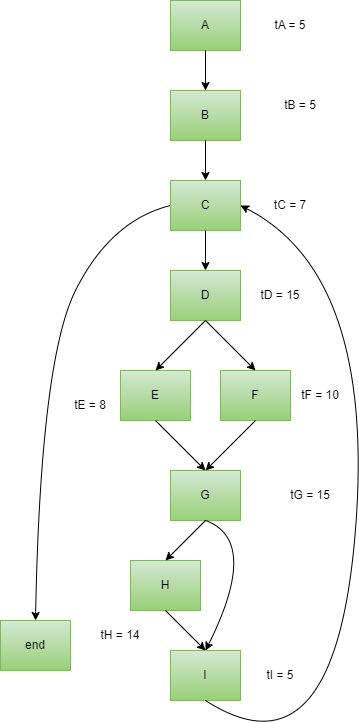
\includegraphics[height=350px]{images/Ass3Q5.png}
        \caption{This is the flow-graph with the execution times of each segment used to calclate the WCET bound.}
        \label{fig:path}
    \end{figure}

    The following paths of the loop are found in the flow graph:
    \begin{enumerate}
        \item  $C\rightarrow D\rightarrow F\rightarrow G\rightarrow H\rightarrow I$
        \item $C\rightarrow D\rightarrow F\rightarrow G\rightarrow I$
        \item $C\rightarrow D\rightarrow E\rightarrow G\rightarrow H\rightarrow I$
        \item $C\rightarrow D\rightarrow E\rightarrow G\rightarrow I$
    \end{enumerate}

    Since the first path is infeasible, no further calculations will be done on it. Calculations of the length of the other paths is as follows:
    \begin{enumerate}
        \item N/A
        \item $7+15+10+15+5 = 52$
        \item $7+15+8+15+14+5 = 64$
        \item $7+15+8+15+5 = 50$
    \end{enumerate}

    The longest path is path 3 with a length of 64. The tight upper bound for the loop is 50. Therefore the WCET bound is $64*50 + t_A + t_B = 3210$. This result is smaller than the tree-based calculation by a margin of $100$ cycles.


